\documentclass[10pt,a4paper]{article}
\usepackage[utf8]{inputenc}
\usepackage[italian]{babel}
\usepackage[a4paper]{geometry}
\usepackage{amsmath}
\usepackage{amsthm}
\usepackage{dsfont}
\usepackage{xfrac}
\usepackage{amsfonts}
\usepackage{amssymb}
\usepackage{graphicx}
\usepackage{braket}
\usepackage{mathtools}
\usepackage{hyperref}
\usepackage{enumerate}
\DeclarePairedDelimiterX{\norm}[1]{\lVert}{\rVert}{#1}
\theoremstyle{plain}
\newtheorem{definizione}{Definizione}
\theoremstyle{definition}
\newtheorem{teorema}{Teorema}
\newtheorem{corollario}{Corollario}
\newtheorem{osservazione}{Osservazione}
\newtheorem{esempio}{Esempio}
%%%%%%%INSERIAMO QUI I NUOVI COMANDI %%%%%%%%%%%%%%%%%%%%%%%%%%%%%%%%%%%%%%%%%%%%
\DeclarePairedDelimiterX{\abla}[1]{abla}{abla}{#1}

%%%%%%%QUI VANNO INSERITI IL TITOLO E GLI AUTORI%%%%%%%%%%%%%%%%%%%%%%%%%%%%
\author{Dante Alighieri}
\title{La Divina Commedia}
\date{Qualche giorno del 1312}
\begin{document}
\maketitle
\section{Rette}
Noob math: y=x \\
Better math: $y=x$ \\
In display math:
\[y=x\]
Old math:
$$
y=x
$$
Lista della spesa:
\begin{itemize}
	\item pane
	\begin{itemize}
		\item rosette
		\item baguettes
	\end{itemize}
	\item latte
	\item veleno
\end{itemize}
$$$$ %this should be fixed
lista della spesa numerata:
\begin{enumerate}[\quad\#1]
	\item pane
	\begin{enumerate}[\quad(i)]
		\item rosette
		\item baguettes
	\end{enumerate}
	\item latte
	\item veleno
\end{enumerate}

\begin{osservazione}
	Le rette sono dritte
\end{osservazione}

\begin{osservazione}
	\label{I'm so smart}
	Le rette hanno tanti punti
\end{osservazione}

\begin{equation}
x=55555
\end{equation}

\section{Algebra lineare}
$$
\begin{pmatrix}
	1 & 2 & 3 & 4 \\
	5 & 6 & 7 & 8
\end{pmatrix}
\cdot
\begin{pmatrix}
	1 \\
	2 \\
	3 \\
	4 
\end{pmatrix}
$$
Altre cose

$$
\begin{pmatrix}
	1 & 2 \\
	3 & 4
\end{pmatrix}
\cdot
\begin{pmatrix}
	x \\
	y
\end{pmatrix}
=
\begin{pmatrix}
	0 \\
	10
\end{pmatrix}
$$

$$
\begin{cases}
	1x+2y=0 \\
	3x+4y=10
\end{cases}
$$

Frazioni: \\
tfrac sta dentro il testo $\tfrac{2}{3}$ \\
fancy frac: $\sfrac{2}{3}$ \\


Andrea usa riferimento incrociato, è superefficacie.\\
Osservazione \ref{I'm so smart}\\

In genere si usa il grassetto per indicare i vettori invece che l'overline\\
Norma: $\norm{\mathbf{x}}$
\section{Notes}
Devi scrivere dentro degli ambienti (e.g. document)

\section{Cool stuff}
$$
e^{\pi i} - 1 = 0
$$

detexify.kirelabs.org/classify.html \\

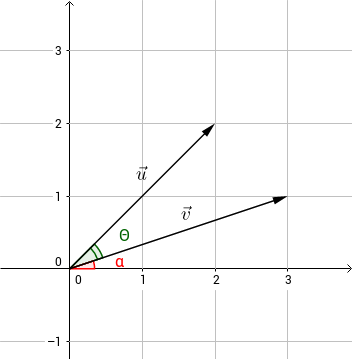
\includegraphics{graph.png}


\end{document}